\section{Data storage and management system}

%%%%%%%%%%%%%%%%%%%%%%%%
\subsection{Data characteristics}

It is the TPC data that drives the requirements for the raw \pdsp data.
The \textit{\pdsp Data Scenarios} spreadsheet~\cite{data_spreadsheet}  %(DUNE DocDB 1086)
provides details on these %above 
numbers and a few alternative running conditions.
Table~\ref{tab:goldi} summarizes the nominal estimates.

\begin{table}[h]
  \centering
  \begin{tabular}[h]{|r|l|}
    \hline
    Parameter & estimate  \\
    \hline
    In-spill trigger rate & 25 Hz \\
    Avg. trigger rate & 10 Hz \\
    Channels & 15,360 \\
    Readout time & 5 ms \\
    Compression & $4\times$ \\
    \hline
    Compressed event & 60 MByte  \\
    Instantaneous rate & 1.5 GByte/sec \\
    Average rate & 600 MByte/sec \\
    \hline
    Total triggers & 52 M \\
    Total volume & 3 PB  \\
    \hline
  \end{tabular}
  \caption{Estimates of nominal raw data parameters driving the design for the raw data storage and management.}
  \label{tab:goldi}
\end{table}

The average trigger rate over the entire beam cycle assumes that one
out-of-spill trigger from the Cosmic Ray Trigger (CRT) system (Section~\ref{sec:beam:muontagger}) 
%cosmic-$\mu$ trigger system 
is acquired
for every in-spill trigger due to the beam.  The assumed compression
factor can be achieved even with similar levels of excess noise as
experienced in the first year of MicroBooNE running~\cite{docdb2089}.
If no excess noise is experienced, as expected, then a compression factor
of 6 -- 8 is expected.  A data-reduction scheme is described in
Section~\ref{sec:datareduc}.
\fixme{data reduction - to remove?}


%%%%%%%%%%%%%%%%%%%%%%%%
\subsection{Raw data flow}
\label{sec:raw_concept}


A conceptual diagram of the raw data flow is presented in
Figure~\ref{fig:raw_concept}.  It reflects the central role of the
CERN storage service \textit{EOS} in the raw data management scheme.
Long-term experience has been gained by the LHC experiments, and EOS
has proven to be performant and reliable.  EOS serves as the staging
area from which the data are committed to CASTOR (a hierarchical
storage management system developed at CERN) and from which data are
transmitted to a number of endpoints including principal data centers
such as Fermilab and others.  It is also used to provide input to DQM
and will be available for personal ad-hoc analyses.

\begin{cdrfigure}[Conceptual diagram of the flow of raw data in \pdsp]{raw_concept}{Conceptual diagram of the flow of raw data in \pdsp} 
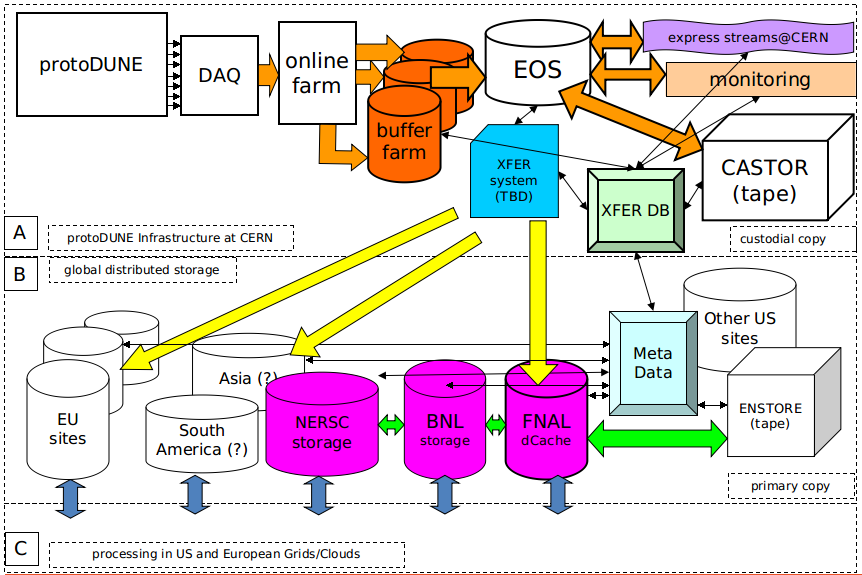
\includegraphics[width=0.9\textwidth]{protoDUNE_raw_data_concept.png}
\end{cdrfigure}


